\documentclass[]{article}
\usepackage{lmodern}
\usepackage{amssymb,amsmath}
\usepackage{ifxetex,ifluatex}
\usepackage{fixltx2e} % provides \textsubscript
\ifnum 0\ifxetex 1\fi\ifluatex 1\fi=0 % if pdftex
  \usepackage[T1]{fontenc}
  \usepackage[utf8]{inputenc}
\else % if luatex or xelatex
  \ifxetex
    \usepackage{mathspec}
  \else
    \usepackage{fontspec}
  \fi
  \defaultfontfeatures{Ligatures=TeX,Scale=MatchLowercase}
\fi
% use upquote if available, for straight quotes in verbatim environments
\IfFileExists{upquote.sty}{\usepackage{upquote}}{}
% use microtype if available
\IfFileExists{microtype.sty}{%
\usepackage{microtype}
\UseMicrotypeSet[protrusion]{basicmath} % disable protrusion for tt fonts
}{}
\usepackage[margin=2.54cm]{geometry}
\usepackage{hyperref}
\hypersetup{unicode=true,
            pdftitle={Assignment 6: Generalized Linear Models},
            pdfauthor={Felipe Raby Amadori},
            pdfborder={0 0 0},
            breaklinks=true}
\urlstyle{same}  % don't use monospace font for urls
\usepackage{color}
\usepackage{fancyvrb}
\newcommand{\VerbBar}{|}
\newcommand{\VERB}{\Verb[commandchars=\\\{\}]}
\DefineVerbatimEnvironment{Highlighting}{Verbatim}{commandchars=\\\{\}}
% Add ',fontsize=\small' for more characters per line
\usepackage{framed}
\definecolor{shadecolor}{RGB}{248,248,248}
\newenvironment{Shaded}{\begin{snugshade}}{\end{snugshade}}
\newcommand{\KeywordTok}[1]{\textcolor[rgb]{0.13,0.29,0.53}{\textbf{#1}}}
\newcommand{\DataTypeTok}[1]{\textcolor[rgb]{0.13,0.29,0.53}{#1}}
\newcommand{\DecValTok}[1]{\textcolor[rgb]{0.00,0.00,0.81}{#1}}
\newcommand{\BaseNTok}[1]{\textcolor[rgb]{0.00,0.00,0.81}{#1}}
\newcommand{\FloatTok}[1]{\textcolor[rgb]{0.00,0.00,0.81}{#1}}
\newcommand{\ConstantTok}[1]{\textcolor[rgb]{0.00,0.00,0.00}{#1}}
\newcommand{\CharTok}[1]{\textcolor[rgb]{0.31,0.60,0.02}{#1}}
\newcommand{\SpecialCharTok}[1]{\textcolor[rgb]{0.00,0.00,0.00}{#1}}
\newcommand{\StringTok}[1]{\textcolor[rgb]{0.31,0.60,0.02}{#1}}
\newcommand{\VerbatimStringTok}[1]{\textcolor[rgb]{0.31,0.60,0.02}{#1}}
\newcommand{\SpecialStringTok}[1]{\textcolor[rgb]{0.31,0.60,0.02}{#1}}
\newcommand{\ImportTok}[1]{#1}
\newcommand{\CommentTok}[1]{\textcolor[rgb]{0.56,0.35,0.01}{\textit{#1}}}
\newcommand{\DocumentationTok}[1]{\textcolor[rgb]{0.56,0.35,0.01}{\textbf{\textit{#1}}}}
\newcommand{\AnnotationTok}[1]{\textcolor[rgb]{0.56,0.35,0.01}{\textbf{\textit{#1}}}}
\newcommand{\CommentVarTok}[1]{\textcolor[rgb]{0.56,0.35,0.01}{\textbf{\textit{#1}}}}
\newcommand{\OtherTok}[1]{\textcolor[rgb]{0.56,0.35,0.01}{#1}}
\newcommand{\FunctionTok}[1]{\textcolor[rgb]{0.00,0.00,0.00}{#1}}
\newcommand{\VariableTok}[1]{\textcolor[rgb]{0.00,0.00,0.00}{#1}}
\newcommand{\ControlFlowTok}[1]{\textcolor[rgb]{0.13,0.29,0.53}{\textbf{#1}}}
\newcommand{\OperatorTok}[1]{\textcolor[rgb]{0.81,0.36,0.00}{\textbf{#1}}}
\newcommand{\BuiltInTok}[1]{#1}
\newcommand{\ExtensionTok}[1]{#1}
\newcommand{\PreprocessorTok}[1]{\textcolor[rgb]{0.56,0.35,0.01}{\textit{#1}}}
\newcommand{\AttributeTok}[1]{\textcolor[rgb]{0.77,0.63,0.00}{#1}}
\newcommand{\RegionMarkerTok}[1]{#1}
\newcommand{\InformationTok}[1]{\textcolor[rgb]{0.56,0.35,0.01}{\textbf{\textit{#1}}}}
\newcommand{\WarningTok}[1]{\textcolor[rgb]{0.56,0.35,0.01}{\textbf{\textit{#1}}}}
\newcommand{\AlertTok}[1]{\textcolor[rgb]{0.94,0.16,0.16}{#1}}
\newcommand{\ErrorTok}[1]{\textcolor[rgb]{0.64,0.00,0.00}{\textbf{#1}}}
\newcommand{\NormalTok}[1]{#1}
\usepackage{graphicx,grffile}
\makeatletter
\def\maxwidth{\ifdim\Gin@nat@width>\linewidth\linewidth\else\Gin@nat@width\fi}
\def\maxheight{\ifdim\Gin@nat@height>\textheight\textheight\else\Gin@nat@height\fi}
\makeatother
% Scale images if necessary, so that they will not overflow the page
% margins by default, and it is still possible to overwrite the defaults
% using explicit options in \includegraphics[width, height, ...]{}
\setkeys{Gin}{width=\maxwidth,height=\maxheight,keepaspectratio}
\IfFileExists{parskip.sty}{%
\usepackage{parskip}
}{% else
\setlength{\parindent}{0pt}
\setlength{\parskip}{6pt plus 2pt minus 1pt}
}
\setlength{\emergencystretch}{3em}  % prevent overfull lines
\providecommand{\tightlist}{%
  \setlength{\itemsep}{0pt}\setlength{\parskip}{0pt}}
\setcounter{secnumdepth}{0}
% Redefines (sub)paragraphs to behave more like sections
\ifx\paragraph\undefined\else
\let\oldparagraph\paragraph
\renewcommand{\paragraph}[1]{\oldparagraph{#1}\mbox{}}
\fi
\ifx\subparagraph\undefined\else
\let\oldsubparagraph\subparagraph
\renewcommand{\subparagraph}[1]{\oldsubparagraph{#1}\mbox{}}
\fi

%%% Use protect on footnotes to avoid problems with footnotes in titles
\let\rmarkdownfootnote\footnote%
\def\footnote{\protect\rmarkdownfootnote}

%%% Change title format to be more compact
\usepackage{titling}

% Create subtitle command for use in maketitle
\newcommand{\subtitle}[1]{
  \posttitle{
    \begin{center}\large#1\end{center}
    }
}

\setlength{\droptitle}{-2em}

  \title{Assignment 6: Generalized Linear Models}
    \pretitle{\vspace{\droptitle}\centering\huge}
  \posttitle{\par}
    \author{Felipe Raby Amadori}
    \preauthor{\centering\large\emph}
  \postauthor{\par}
    \date{}
    \predate{}\postdate{}
  

\begin{document}
\maketitle

\subsection{OVERVIEW}\label{overview}

This exercise accompanies the lessons in Environmental Data Analytics
(ENV872L) on generalized linear models.

\subsection{Directions}\label{directions}

\begin{enumerate}
\def\labelenumi{\arabic{enumi}.}
\tightlist
\item
  Change ``Student Name'' on line 3 (above) with your name.
\item
  Use the lesson as a guide. It contains code that can be modified to
  complete the assignment.
\item
  Work through the steps, \textbf{creating code and output} that fulfill
  each instruction.
\item
  Be sure to \textbf{answer the questions} in this assignment document.
  Space for your answers is provided in this document and is indicated
  by the ``\textgreater{}'' character. If you need a second paragraph be
  sure to start the first line with ``\textgreater{}''. You should
  notice that the answer is highlighted in green by RStudio.
\item
  When you have completed the assignment, \textbf{Knit} the text and
  code into a single PDF file. You will need to have the correct
  software installed to do this (see Software Installation Guide) Press
  the \texttt{Knit} button in the RStudio scripting panel. This will
  save the PDF output in your Assignments folder.
\item
  After Knitting, please submit the completed exercise (PDF file) to the
  dropbox in Sakai. Please add your last name into the file name (e.g.,
  ``Salk\_A06\_GLMs.pdf'') prior to submission.
\end{enumerate}

The completed exercise is due on Tuesday, 26 February, 2019 before class
begins.

\subsection{Set up your session}\label{set-up-your-session}

\begin{enumerate}
\def\labelenumi{\arabic{enumi}.}
\item
  Set up your session. Upload the EPA Ecotox dataset for Neonicotinoids
  and the NTL-LTER raw data file for chemistry/physics.
\item
  Build a ggplot theme and set it as your default theme.
\end{enumerate}

\begin{Shaded}
\begin{Highlighting}[]
\NormalTok{knitr}\OperatorTok{::}\NormalTok{opts_chunk}\OperatorTok{$}\KeywordTok{set}\NormalTok{(}\DataTypeTok{echo =} \OtherTok{TRUE}\NormalTok{, }\DataTypeTok{message =} \OtherTok{FALSE}\NormalTok{, }\DataTypeTok{warning =} \OtherTok{FALSE}\NormalTok{, }\DataTypeTok{eval=}\OtherTok{TRUE}\NormalTok{)}

\CommentTok{#1}
\KeywordTok{getwd}\NormalTok{()}
\end{Highlighting}
\end{Shaded}

\begin{verbatim}
## [1] "C:/Users/Felipe/OneDrive - Duke University/1. DUKE/1. Ramos 2 Semestre/EOS-872 Env. Data Analytics/Environmental_Data_Analytics"
\end{verbatim}

\begin{Shaded}
\begin{Highlighting}[]
\CommentTok{#install.packages('FSA')}
\KeywordTok{library}\NormalTok{(FSA)}
\end{Highlighting}
\end{Shaded}

\begin{verbatim}
## ## FSA v0.8.22. See citation('FSA') if used in publication.
## ## Run fishR() for related website and fishR('IFAR') for related book.
\end{verbatim}

\begin{Shaded}
\begin{Highlighting}[]
\KeywordTok{library}\NormalTok{(tidyverse)}
\end{Highlighting}
\end{Shaded}

\begin{verbatim}
## -- Attaching packages ----------------------------------------- tidyverse 1.2.1 --
\end{verbatim}

\begin{verbatim}
## v ggplot2 3.0.0     v purrr   0.2.5
## v tibble  1.4.2     v dplyr   0.7.6
## v tidyr   0.8.1     v stringr 1.3.1
## v readr   1.1.1     v forcats 0.3.0
\end{verbatim}

\begin{verbatim}
## -- Conflicts -------------------------------------------- tidyverse_conflicts() --
## x dplyr::filter() masks stats::filter()
## x dplyr::lag()    masks stats::lag()
\end{verbatim}

\begin{Shaded}
\begin{Highlighting}[]
\KeywordTok{library}\NormalTok{(RColorBrewer)}
\KeywordTok{library}\NormalTok{(ggpubr)}
\end{Highlighting}
\end{Shaded}

\begin{verbatim}
## Loading required package: magrittr
\end{verbatim}

\begin{verbatim}
## 
## Attaching package: 'magrittr'
\end{verbatim}

\begin{verbatim}
## The following object is masked from 'package:purrr':
## 
##     set_names
\end{verbatim}

\begin{verbatim}
## The following object is masked from 'package:tidyr':
## 
##     extract
\end{verbatim}

\begin{Shaded}
\begin{Highlighting}[]
\KeywordTok{library}\NormalTok{(viridis)}
\end{Highlighting}
\end{Shaded}

\begin{verbatim}
## Loading required package: viridisLite
\end{verbatim}

\begin{Shaded}
\begin{Highlighting}[]
\KeywordTok{library}\NormalTok{(colormap)}

\NormalTok{EPA_Ecotox_Neonicotinoids <-}\StringTok{ }\KeywordTok{read.csv}\NormalTok{(}\StringTok{"./Data/Raw/ECOTOX_Neonicotinoids_Mortality_raw.csv"}\NormalTok{)}

\NormalTok{NTL_TER_raw_chemistryphysics <-}\StringTok{ }\KeywordTok{read.csv}\NormalTok{(}\StringTok{"./Data/Raw/NTL-LTER_Lake_ChemistryPhysics_Raw.csv"}\NormalTok{)}

\CommentTok{#2}
\NormalTok{felipe_theme <-}\StringTok{ }\KeywordTok{theme_light}\NormalTok{(}\DataTypeTok{base_size =} \DecValTok{12}\NormalTok{) }\OperatorTok{+}
\StringTok{  }\KeywordTok{theme}\NormalTok{(}\DataTypeTok{axis.text =} \KeywordTok{element_text}\NormalTok{(}\DataTypeTok{color =} \StringTok{"grey8"}\NormalTok{), }
        \DataTypeTok{legend.position =} \StringTok{"right"}\NormalTok{, }\DataTypeTok{plot.title =} \KeywordTok{element_text}\NormalTok{(}\DataTypeTok{hjust =} \FloatTok{0.5}\NormalTok{)) }
\KeywordTok{theme_set}\NormalTok{(felipe_theme)}
\end{Highlighting}
\end{Shaded}

\subsection{Neonicotinoids test}\label{neonicotinoids-test}

Research question: Were studies on various neonicotinoid chemicals
conducted in different years?

\begin{enumerate}
\def\labelenumi{\arabic{enumi}.}
\setcounter{enumi}{2}
\item
  Generate a line of code to determine how many different chemicals are
  listed in the Chemical.Name column.
\item
  Are the publication years associated with each chemical
  well-approximated by a normal distribution? Run the appropriate test
  and also generate a frequency polygon to illustrate the distribution
  of counts for each year, divided by chemical name. Bonus points if you
  can generate the results of your test from a pipe function. No need to
  make this graph pretty.
\item
  Is there equal variance among the publication years for each chemical?
  Hint: var.test is not the correct function.
\end{enumerate}

\begin{Shaded}
\begin{Highlighting}[]
\CommentTok{#3}
\KeywordTok{levels}\NormalTok{(EPA_Ecotox_Neonicotinoids}\OperatorTok{$}\NormalTok{Chemical.Name)}
\end{Highlighting}
\end{Shaded}

\begin{verbatim}
## [1] "Acetamiprid"  "Clothianidin" "Dinotefuran"  "Imidacloprid"
## [5] "Imidaclothiz" "Nitenpyram"   "Nithiazine"   "Thiacloprid" 
## [9] "Thiamethoxam"
\end{verbatim}

\begin{Shaded}
\begin{Highlighting}[]
\KeywordTok{length}\NormalTok{(}\KeywordTok{levels}\NormalTok{(EPA_Ecotox_Neonicotinoids}\OperatorTok{$}\NormalTok{Chemical.Name))}
\end{Highlighting}
\end{Shaded}

\begin{verbatim}
## [1] 9
\end{verbatim}

\begin{Shaded}
\begin{Highlighting}[]
\CommentTok{# Numbers of different chemicals listed in the Chemical.Name column.}

\CommentTok{#4}
\CommentTok{# To evaluate assumption of normal distribution we run the Shapiro-Wilk test }
\CommentTok{# for each chemical, where the null hypothesis is that the data come from a normal distribution.}

\KeywordTok{shapiro.test}\NormalTok{(EPA_Ecotox_Neonicotinoids}\OperatorTok{$}\NormalTok{Pub..Year[EPA_Ecotox_Neonicotinoids}\OperatorTok{$}\NormalTok{Chemical.Name}
                                                 \OperatorTok{==}\StringTok{ "Acetamiprid"}\NormalTok{])}
\end{Highlighting}
\end{Shaded}

\begin{verbatim}
## 
##  Shapiro-Wilk normality test
## 
## data:  EPA_Ecotox_Neonicotinoids$Pub..Year[EPA_Ecotox_Neonicotinoids$Chemical.Name ==     "Acetamiprid"]
## W = 0.90191, p-value = 5.706e-08
\end{verbatim}

\begin{Shaded}
\begin{Highlighting}[]
\CommentTok{# Acetamiprid data are significantly different from }
\CommentTok{# a normal distribution (Shapiro-Wilk normality test, W = 0.90191, p-value = 5.706e-08).}

\KeywordTok{shapiro.test}\NormalTok{(EPA_Ecotox_Neonicotinoids}\OperatorTok{$}\NormalTok{Pub..Year[EPA_Ecotox_Neonicotinoids}\OperatorTok{$}\NormalTok{Chemical.Name }
                                                 \OperatorTok{==}\StringTok{ "Clothianidin"}\NormalTok{])}
\end{Highlighting}
\end{Shaded}

\begin{verbatim}
## 
##  Shapiro-Wilk normality test
## 
## data:  EPA_Ecotox_Neonicotinoids$Pub..Year[EPA_Ecotox_Neonicotinoids$Chemical.Name ==     "Clothianidin"]
## W = 0.69577, p-value = 4.287e-11
\end{verbatim}

\begin{Shaded}
\begin{Highlighting}[]
\CommentTok{# Clothianidin data are significantly different from }
\CommentTok{# a normal distribution (Shapiro-Wilk normality test, W = 0.69577, p-value = 4.287e-11).}

\KeywordTok{shapiro.test}\NormalTok{(EPA_Ecotox_Neonicotinoids}\OperatorTok{$}\NormalTok{Pub..Year[EPA_Ecotox_Neonicotinoids}\OperatorTok{$}\NormalTok{Chemical.Name }
                                                 \OperatorTok{==}\StringTok{ "Dinotefuran"}\NormalTok{])}
\end{Highlighting}
\end{Shaded}

\begin{verbatim}
## 
##  Shapiro-Wilk normality test
## 
## data:  EPA_Ecotox_Neonicotinoids$Pub..Year[EPA_Ecotox_Neonicotinoids$Chemical.Name ==     "Dinotefuran"]
## W = 0.82848, p-value = 8.83e-07
\end{verbatim}

\begin{Shaded}
\begin{Highlighting}[]
\CommentTok{# Dinotefuran data are significantly different from }
\CommentTok{# a normal distribution (Shapiro-Wilk normality test, W = 0.82848, p-value = 8.83e-07).}

\KeywordTok{shapiro.test}\NormalTok{(EPA_Ecotox_Neonicotinoids}\OperatorTok{$}\NormalTok{Pub..Year[EPA_Ecotox_Neonicotinoids}\OperatorTok{$}\NormalTok{Chemical.Name }
                                                 \OperatorTok{==}\StringTok{ "Imidacloprid"}\NormalTok{])}
\end{Highlighting}
\end{Shaded}

\begin{verbatim}
## 
##  Shapiro-Wilk normality test
## 
## data:  EPA_Ecotox_Neonicotinoids$Pub..Year[EPA_Ecotox_Neonicotinoids$Chemical.Name ==     "Imidacloprid"]
## W = 0.88178, p-value < 2.2e-16
\end{verbatim}

\begin{Shaded}
\begin{Highlighting}[]
\CommentTok{# Imidacloprid data are significantly different from }
\CommentTok{# a normal distribution (Shapiro-Wilk normality test, W = 0.88178, p-value < 2.2e-16).}

\KeywordTok{shapiro.test}\NormalTok{(EPA_Ecotox_Neonicotinoids}\OperatorTok{$}\NormalTok{Pub..Year[EPA_Ecotox_Neonicotinoids}\OperatorTok{$}\NormalTok{Chemical.Name }
                                                 \OperatorTok{==}\StringTok{ "Imidaclothiz"}\NormalTok{])}
\end{Highlighting}
\end{Shaded}

\begin{verbatim}
## 
##  Shapiro-Wilk normality test
## 
## data:  EPA_Ecotox_Neonicotinoids$Pub..Year[EPA_Ecotox_Neonicotinoids$Chemical.Name ==     "Imidaclothiz"]
## W = 0.68429, p-value = 0.00093
\end{verbatim}

\begin{Shaded}
\begin{Highlighting}[]
\CommentTok{# Imidaclothiz data are significantly different from }
\CommentTok{# a normal distribution (Shapiro-Wilk normality test, W = 0.68429, p-value = 0.00093).}

\KeywordTok{shapiro.test}\NormalTok{(EPA_Ecotox_Neonicotinoids}\OperatorTok{$}\NormalTok{Pub..Year[EPA_Ecotox_Neonicotinoids}\OperatorTok{$}\NormalTok{Chemical.Name }
                                                 \OperatorTok{==}\StringTok{ "Nitenpyram"}\NormalTok{])}
\end{Highlighting}
\end{Shaded}

\begin{verbatim}
## 
##  Shapiro-Wilk normality test
## 
## data:  EPA_Ecotox_Neonicotinoids$Pub..Year[EPA_Ecotox_Neonicotinoids$Chemical.Name ==     "Nitenpyram"]
## W = 0.79592, p-value = 0.0005686
\end{verbatim}

\begin{Shaded}
\begin{Highlighting}[]
\CommentTok{# Nitenpyram data are significantly different from }
\CommentTok{# a normal distribution (Shapiro-Wilk normality test, W = 0.79592, p-value = 0.0005686).}

\KeywordTok{shapiro.test}\NormalTok{(EPA_Ecotox_Neonicotinoids}\OperatorTok{$}\NormalTok{Pub..Year[EPA_Ecotox_Neonicotinoids}\OperatorTok{$}\NormalTok{Chemical.Name }
                                                 \OperatorTok{==}\StringTok{ "Nithiazine"}\NormalTok{])}
\end{Highlighting}
\end{Shaded}

\begin{verbatim}
## 
##  Shapiro-Wilk normality test
## 
## data:  EPA_Ecotox_Neonicotinoids$Pub..Year[EPA_Ecotox_Neonicotinoids$Chemical.Name ==     "Nithiazine"]
## W = 0.75938, p-value = 0.0001235
\end{verbatim}

\begin{Shaded}
\begin{Highlighting}[]
\CommentTok{# Nithiazine data are significantly different from }
\CommentTok{# a normal distribution (Shapiro-Wilk normality test, W = 0.75938, p-value = 0.0001235).}

\KeywordTok{shapiro.test}\NormalTok{(EPA_Ecotox_Neonicotinoids}\OperatorTok{$}\NormalTok{Pub..Year[EPA_Ecotox_Neonicotinoids}\OperatorTok{$}\NormalTok{Chemical.Name }
                                                 \OperatorTok{==}\StringTok{ "Thiacloprid"}\NormalTok{])}
\end{Highlighting}
\end{Shaded}

\begin{verbatim}
## 
##  Shapiro-Wilk normality test
## 
## data:  EPA_Ecotox_Neonicotinoids$Pub..Year[EPA_Ecotox_Neonicotinoids$Chemical.Name ==     "Thiacloprid"]
## W = 0.7669, p-value = 1.118e-11
\end{verbatim}

\begin{Shaded}
\begin{Highlighting}[]
\CommentTok{# Thiacloprid data are significantly different from }
\CommentTok{# a normal distribution (Shapiro-Wilk normality test, W = 0.7669, p-value = 1.118e-11).}

\KeywordTok{shapiro.test}\NormalTok{(EPA_Ecotox_Neonicotinoids}\OperatorTok{$}\NormalTok{Pub..Year[EPA_Ecotox_Neonicotinoids}\OperatorTok{$}\NormalTok{Chemical.Name }
                                                 \OperatorTok{==}\StringTok{ "Thiamethoxam"}\NormalTok{])}
\end{Highlighting}
\end{Shaded}

\begin{verbatim}
## 
##  Shapiro-Wilk normality test
## 
## data:  EPA_Ecotox_Neonicotinoids$Pub..Year[EPA_Ecotox_Neonicotinoids$Chemical.Name ==     "Thiamethoxam"]
## W = 0.7071, p-value < 2.2e-16
\end{verbatim}

\begin{Shaded}
\begin{Highlighting}[]
\CommentTok{# Thiamethoxam data are significantly different from }
\CommentTok{# a normal distribution (Shapiro-Wilk normality test, W = 0.7071, p-value < 2.2e-16).}

\CommentTok{#Graphic Analysis}
\KeywordTok{ggplot}\NormalTok{(EPA_Ecotox_Neonicotinoids, }\KeywordTok{aes}\NormalTok{(}\DataTypeTok{x =}\NormalTok{ Pub..Year, }\DataTypeTok{color =}\NormalTok{ Chemical.Name)) }\OperatorTok{+}
\StringTok{  }\KeywordTok{geom_freqpoly}\NormalTok{(}\DataTypeTok{stat =} \StringTok{"count"}\NormalTok{)}
\end{Highlighting}
\end{Shaded}

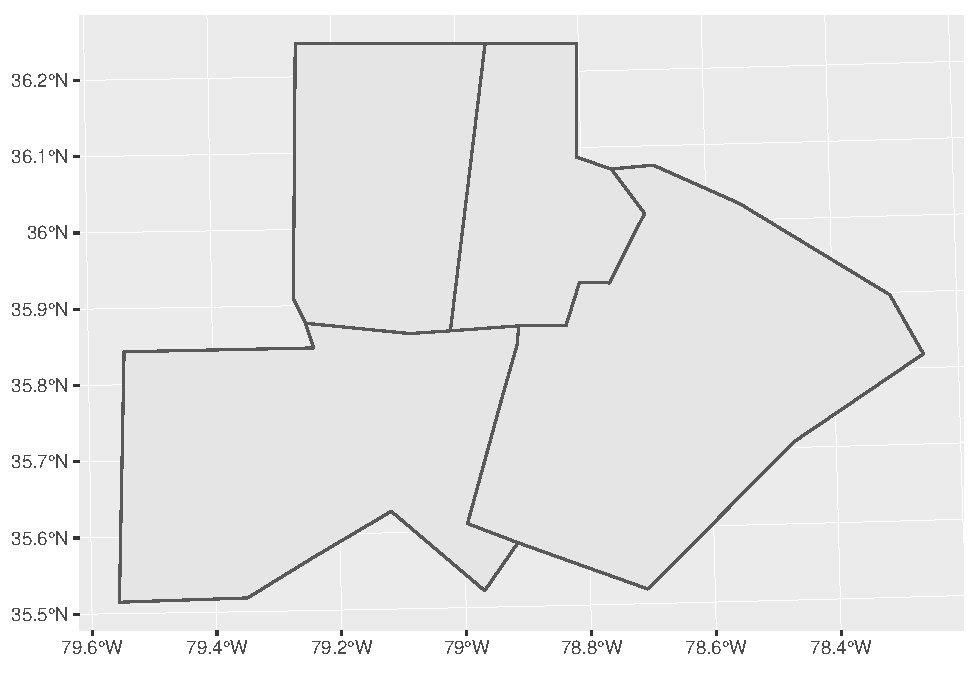
\includegraphics{A06_GLMs_files/figure-latex/unnamed-chunk-2-1.pdf}

\begin{Shaded}
\begin{Highlighting}[]
\CommentTok{# The graphic analysis gave as a result that the assumption that the }
\CommentTok{# data are normally distributed is not met. The data don't have a single peak }
\CommentTok{# around the mean and has a longer tail towards the earlier years.}

\CommentTok{#5}
\CommentTok{# We perform a Bartlett's test of the null hypothesis that the variances in each }
\CommentTok{# of the groups are the same.}
\KeywordTok{bartlett.test}\NormalTok{(EPA_Ecotox_Neonicotinoids}\OperatorTok{$}\NormalTok{Pub..Year }\OperatorTok{~}\StringTok{ }\NormalTok{EPA_Ecotox_Neonicotinoids}\OperatorTok{$}\NormalTok{Chemical.Name)}
\end{Highlighting}
\end{Shaded}

\begin{verbatim}
## 
##  Bartlett test of homogeneity of variances
## 
## data:  EPA_Ecotox_Neonicotinoids$Pub..Year by EPA_Ecotox_Neonicotinoids$Chemical.Name
## Bartlett's K-squared = 139.59, df = 8, p-value < 2.2e-16
\end{verbatim}

\begin{Shaded}
\begin{Highlighting}[]
\CommentTok{# The variance of the data are significantly different from }
\CommentTok{# each other (Bartlett test, K-squared = 139.59, df = 8, p-value < 2.2e-16).}
\end{Highlighting}
\end{Shaded}

\begin{enumerate}
\def\labelenumi{\arabic{enumi}.}
\setcounter{enumi}{5}
\tightlist
\item
  Based on your results, which test would you choose to run to answer
  your research question?
\end{enumerate}

\begin{quote}
ANSWER: Considering that the data are not well-approximated by a normal
distribution and there is not equal variance among the publication years
for each chemical, we choose the Kruskal-Wallis test, which is the
non-parametric counterpart to the one-way ANOVA.
\end{quote}

\begin{enumerate}
\def\labelenumi{\arabic{enumi}.}
\setcounter{enumi}{6}
\item
  Run this test below.
\item
  Generate a boxplot representing the range of publication years for
  each chemical. Adjust your graph to make it pretty.
\end{enumerate}

\begin{Shaded}
\begin{Highlighting}[]
\CommentTok{#7}
\NormalTok{PubYear.kW_test <-}\StringTok{ }\KeywordTok{kruskal.test}\NormalTok{(}
\NormalTok{  EPA_Ecotox_Neonicotinoids}\OperatorTok{$}\NormalTok{Pub..Year }\OperatorTok{~}\StringTok{ }\NormalTok{EPA_Ecotox_Neonicotinoids}\OperatorTok{$}\NormalTok{Chemical.Name)}
\NormalTok{PubYear.kW_test}
\end{Highlighting}
\end{Shaded}

\begin{verbatim}
## 
##  Kruskal-Wallis rank sum test
## 
## data:  EPA_Ecotox_Neonicotinoids$Pub..Year by EPA_Ecotox_Neonicotinoids$Chemical.Name
## Kruskal-Wallis chi-squared = 134.15, df = 8, p-value < 2.2e-16
\end{verbatim}

\begin{Shaded}
\begin{Highlighting}[]
\CommentTok{# There are significant differences between the number of studies on various}
\CommentTok{# neonicotinoid chemicals conducted in different years (Kruskal-Wallis chi-squared =}
\CommentTok{# 134.15, df = 8, p-value < 2.2e-16). Nevertheless, we don't know which groups differ}
\CommentTok{# from each other.}

\KeywordTok{dunnTest}\NormalTok{(EPA_Ecotox_Neonicotinoids}\OperatorTok{$}\NormalTok{Pub..Year, EPA_Ecotox_Neonicotinoids}\OperatorTok{$}\NormalTok{Chemical.Name)}
\end{Highlighting}
\end{Shaded}

\begin{verbatim}
##                     Comparison          Z      P.unadj        P.adj
## 1   Acetamiprid - Clothianidin -3.0388079 2.375163e-03 4.037777e-02
## 2    Acetamiprid - Dinotefuran  2.1172089 3.424212e-02 4.109054e-01
## 3   Clothianidin - Dinotefuran  4.4060765 1.052598e-05 2.420975e-04
## 4   Acetamiprid - Imidacloprid -4.0204987 5.807507e-05 1.277651e-03
## 5  Clothianidin - Imidacloprid  0.5068899 6.122321e-01 1.000000e+00
## 6   Dinotefuran - Imidacloprid -5.2140290 1.847826e-07 4.989129e-06
## 7   Acetamiprid - Imidaclothiz -1.8052932 7.102881e-02 7.813169e-01
## 8  Clothianidin - Imidaclothiz -0.5166649 6.053901e-01 1.000000e+00
## 9   Dinotefuran - Imidaclothiz -2.6586494 7.845456e-03 1.176818e-01
## 10 Imidacloprid - Imidaclothiz -0.7284284 4.663514e-01 1.000000e+00
## 11    Acetamiprid - Nitenpyram -4.5018639 6.736012e-06 1.616643e-04
## 12   Clothianidin - Nitenpyram -2.4936264 1.264456e-02 1.770238e-01
## 13    Dinotefuran - Nitenpyram -5.4527796 4.958852e-08 1.388479e-06
## 14   Imidacloprid - Nitenpyram -3.0634837 2.187761e-03 3.937970e-02
## 15   Imidaclothiz - Nitenpyram -1.0897204 2.758363e-01 1.000000e+00
## 16    Acetamiprid - Nithiazine  5.6425299 1.675694e-08 4.859513e-07
## 17   Clothianidin - Nithiazine  7.1473251 8.848514e-13 2.831524e-11
## 18    Dinotefuran - Nithiazine  3.8693508 1.091255e-04 2.291636e-03
## 19   Imidacloprid - Nithiazine  7.7286349 1.087060e-14 3.804708e-13
## 20   Imidaclothiz - Nithiazine  4.8473136 1.251445e-06 3.253758e-05
## 21     Nitenpyram - Nithiazine  7.7099812 1.258363e-14 4.278434e-13
## 22   Acetamiprid - Thiacloprid -3.2225618 1.270497e-03 2.413945e-02
## 23  Clothianidin - Thiacloprid  0.1414916 8.874816e-01 8.874816e-01
## 24   Dinotefuran - Thiacloprid -4.6025295 4.173904e-06 1.043476e-04
## 25  Imidacloprid - Thiacloprid -0.3888712 6.973714e-01 1.000000e+00
## 26  Imidaclothiz - Thiacloprid  0.5870686 5.571576e-01 1.000000e+00
## 27    Nitenpyram - Thiacloprid  2.6709745 7.563140e-03 1.210102e-01
## 28    Nithiazine - Thiacloprid -7.3166886 2.541647e-13 8.387437e-12
## 29  Acetamiprid - Thiamethoxam -5.8898861 3.864618e-09 1.159385e-07
## 30 Clothianidin - Thiamethoxam -1.7587256 7.862413e-02 7.862413e-01
## 31  Dinotefuran - Thiamethoxam -6.6762123 2.451967e-11 7.601098e-10
## 32 Imidacloprid - Thiamethoxam -3.5327039 4.113329e-04 8.226657e-03
## 33 Imidaclothiz - Thiamethoxam -0.1886278 8.503846e-01 1.000000e+00
## 34   Nitenpyram - Thiamethoxam  1.5927766 1.112103e-01 1.000000e+00
## 35   Nithiazine - Thiamethoxam -8.7224129 2.723352e-18 9.804067e-17
## 36  Thiacloprid - Thiamethoxam -2.1461156 3.186376e-02 4.142288e-01
\end{verbatim}

\begin{Shaded}
\begin{Highlighting}[]
\CommentTok{# Groups that differ}
\CommentTok{# Acetamiprid - Clothianidin (Dunn Test, Z=-3.0388079, p<0.05)}
\CommentTok{# Clothianidin - Dinotefuran  (Dunn Test, Z=4.4060765, p<0.05)}
\CommentTok{# Acetamiprid - Imidacloprid (Dunn Test, Z=-4.0204987, p<0.05)}
\CommentTok{# Dinotefuran - Imidacloprid (Dunn Test, Z=-5.2140290, p<0.05)}
\CommentTok{# Acetamiprid - Nitenpyram (Dunn Test, Z=-4.5018639, p<0.05)}
\CommentTok{# Dinotefuran - Nitenpyram (Dunn Test, Z=-5.4527796, p<0.05)}
\CommentTok{# Imidacloprid - Nitenpyram (Dunn Test, Z=-3.0634837, p<0.05)}
\CommentTok{# Acetamiprid - Nithiazine (Dunn Test, Z=5.6425299, p<0.05)}
\CommentTok{# Clothianidin - Nithiazine (Dunn Test, Z=7.1473251, p<0.05)}
\CommentTok{# Dinotefuran - Nithiazine (Dunn Test, Z=3.8693508, p<0.05) }
\CommentTok{# Imidacloprid - Nithiazine (Dunn Test, Z=7.7286349, p<0.05) }
\CommentTok{# Imidaclothiz - Nithiazine (Dunn Test, Z=4.8473136, p<0.05)}
\CommentTok{# Nitenpyram - Nithiazine (Dunn Test, Z=7.7099812, p<0.05)}
\CommentTok{# Acetamiprid - Thiacloprid (Dunn Test, Z=-3.2225618, p<0.05) }
\CommentTok{# Dinotefuran - Thiacloprid (Dunn Test, Z=-4.6025295, p<0.05)  }
\CommentTok{# Nithiazine - Thiacloprid (Dunn Test, Z=-7.3166886, p<0.05)  }
\CommentTok{# Acetamiprid - Thiamethoxam (Dunn Test, Z=-5.8898861, p<0.05) }
\CommentTok{# Dinotefuran - Thiamethoxam (Dunn Test, Z=-6.6762123, p<0.05)  }
\CommentTok{# Imidacloprid - Thiamethoxam (Dunn Test, Z=-3.5327039, p<0.05) }
\CommentTok{# Nithiazine - Thiamethoxam (Dunn Test, Z=-8.7224129, p<0.05)  }

\CommentTok{#8}
\CommentTok{#Plot}
\NormalTok{EPA_Ecotox_Neon_Plot <-}\StringTok{ }\KeywordTok{ggplot}\NormalTok{(EPA_Ecotox_Neonicotinoids, }
                               \KeywordTok{aes}\NormalTok{(}\DataTypeTok{x =}\NormalTok{ Chemical.Name, }\DataTypeTok{y =}\NormalTok{ Pub..Year, }
                                   \DataTypeTok{fill =}\NormalTok{ Chemical.Name)) }\OperatorTok{+}
\StringTok{  }\KeywordTok{geom_boxplot}\NormalTok{() }\OperatorTok{+}
\StringTok{  }\KeywordTok{theme}\NormalTok{(}\DataTypeTok{axis.text.x =} \KeywordTok{element_text}\NormalTok{(}\DataTypeTok{angle =} \DecValTok{45}\NormalTok{, }\DataTypeTok{hjust =} \DecValTok{1}\NormalTok{)) }\OperatorTok{+}
\StringTok{  }\KeywordTok{scale_fill_brewer}\NormalTok{(}\DataTypeTok{palette =} \StringTok{"Set1"}\NormalTok{) }\OperatorTok{+}
\StringTok{  }\KeywordTok{guides}\NormalTok{(}\DataTypeTok{fill=}\OtherTok{FALSE}\NormalTok{) }\OperatorTok{+}
\StringTok{  }\KeywordTok{xlab}\NormalTok{(}\KeywordTok{expression}\NormalTok{(}\StringTok{"Chemical Name"}\NormalTok{)) }\OperatorTok{+}
\StringTok{  }\KeywordTok{ylab}\NormalTok{(}\KeywordTok{expression}\NormalTok{(}\StringTok{"Year"}\NormalTok{)) }\OperatorTok{+}
\StringTok{  }\KeywordTok{ggtitle}\NormalTok{(}\StringTok{"Range of publication years by chemical"}\NormalTok{)}
\KeywordTok{print}\NormalTok{(EPA_Ecotox_Neon_Plot)}
\end{Highlighting}
\end{Shaded}

\includegraphics{A06_GLMs_files/figure-latex/unnamed-chunk-3-1.pdf}

\begin{enumerate}
\def\labelenumi{\arabic{enumi}.}
\setcounter{enumi}{8}
\tightlist
\item
  How would you summarize the conclusion of your analysis? Include a
  sentence summarizing your findings and include the results of your
  test in parentheses at the end of the sentence.
\end{enumerate}

\begin{quote}
ANSWER: There are significant differences between the number of studies
on various neonicotinoid chemicals conducted in different years
(Kruskal-Wallis chi-squared = 134.15, df = 8, p-value \textless{}
2.2e-16). the number of studies on various neonicotinoid chemicals
conducted in different years that differ from each other are:
\end{quote}

\begin{quote}
Acetamiprid - Clothianidin (Dunn Test, Z=-3.0388079, p\textless{}0.05)\\
Clothianidin - Dinotefuran (Dunn Test, Z=4.4060765, p\textless{}0.05)\\
Acetamiprid - Imidacloprid (Dunn Test, Z=-4.0204987, p\textless{}0.05)\\
Dinotefuran - Imidacloprid (Dunn Test, Z=-5.2140290, p\textless{}0.05)\\
Acetamiprid - Nitenpyram (Dunn Test, Z=-4.5018639, p\textless{}0.05)\\
Dinotefuran - Nitenpyram (Dunn Test, Z=-5.4527796, p\textless{}0.05)\\
Imidacloprid - Nitenpyram (Dunn Test, Z=-3.0634837, p\textless{}0.05)\\
Acetamiprid - Nithiazine (Dunn Test, Z=5.6425299, p\textless{}0.05)\\
Clothianidin - Nithiazine (Dunn Test, Z=7.1473251, p\textless{}0.05)\\
Dinotefuran - Nithiazine (Dunn Test, Z=3.8693508, p\textless{}0.05)\\
Imidacloprid - Nithiazine (Dunn Test, Z=7.7286349, p\textless{}0.05)\\
Imidaclothiz - Nithiazine (Dunn Test, Z=4.8473136, p\textless{}0.05)\\
Nitenpyram - Nithiazine (Dunn Test, Z=7.7099812, p\textless{}0.05)\\
Acetamiprid - Thiacloprid (Dunn Test, Z=-3.2225618, p\textless{}0.05)\\
Dinotefuran - Thiacloprid (Dunn Test, Z=-4.6025295, p\textless{}0.05)\\
Nithiazine - Thiacloprid (Dunn Test, Z=-7.3166886, p\textless{}0.05)\\
Acetamiprid - Thiamethoxam (Dunn Test, Z=-5.8898861, p\textless{}0.05)\\
Dinotefuran - Thiamethoxam (Dunn Test, Z=-6.6762123, p\textless{}0.05)\\
Imidacloprid - Thiamethoxam (Dunn Test, Z=-3.5327039,
p\textless{}0.05)\\
Nithiazine - Thiamethoxam (Dunn Test, Z=-8.7224129, p\textless{}0.05)
\end{quote}

\subsection{NTL-LTER test}\label{ntl-lter-test}

Research question: What is the best set of predictors for lake
temperatures in July across the monitoring period at the North Temperate
Lakes LTER?

\begin{enumerate}
\def\labelenumi{\arabic{enumi}.}
\setcounter{enumi}{10}
\tightlist
\item
  Wrangle your NTL-LTER dataset with a pipe function so that it contains
  only the following criteria:
\end{enumerate}

\begin{itemize}
\tightlist
\item
  Only dates in July (hint: use the daynum column). No need to consider
  leap years.
\item
  Only the columns: lakename, year4, daynum, depth, temperature\_C
\item
  Only complete cases (i.e., remove NAs)
\end{itemize}

\begin{enumerate}
\def\labelenumi{\arabic{enumi}.}
\setcounter{enumi}{11}
\tightlist
\item
  Run an AIC to determine what set of explanatory variables (year4,
  daynum, depth) is best suited to predict temperature. Run a multiple
  regression on the recommended set of variables.
\end{enumerate}

\begin{Shaded}
\begin{Highlighting}[]
\CommentTok{#11}
\NormalTok{NTL_TER_raw_chemistryphysics}\OperatorTok{$}\NormalTok{sampledate <-}
\StringTok{  }\KeywordTok{as.Date}\NormalTok{(NTL_TER_raw_chemistryphysics}\OperatorTok{$}\NormalTok{sampledate, }\DataTypeTok{format =} \StringTok{"%m/%d/%y"}\NormalTok{)}

\NormalTok{NTL_TER_raw_chemistryphysics}\OperatorTok{$}\NormalTok{sampledate <-}
\StringTok{  }\KeywordTok{format}\NormalTok{(NTL_TER_raw_chemistryphysics}\OperatorTok{$}\NormalTok{sampledate, }\StringTok{"%m"}\NormalTok{)}

\NormalTok{NTL_LTER_test <-}\StringTok{ }\NormalTok{NTL_TER_raw_chemistryphysics }\OperatorTok
\StringTok{  }\KeywordTok{filter}\NormalTok{(sampledate }\OperatorTok{==}\StringTok{ "07"}\NormalTok{) }\OperatorTok
\StringTok{  }\KeywordTok{select}\NormalTok{(lakename}\OperatorTok{:}\NormalTok{daynum, depth, temperature_C) }\OperatorTok
\StringTok{  }\KeywordTok{na.omit}\NormalTok{()}

\CommentTok{#12}
\NormalTok{NTL_LTER_AIC <-}\StringTok{ }\KeywordTok{lm}\NormalTok{(}\DataTypeTok{data =}\NormalTok{ NTL_LTER_test, temperature_C }\OperatorTok{~}\StringTok{ }\NormalTok{year4 }\OperatorTok{+}\StringTok{ }\NormalTok{daynum }\OperatorTok{+}\StringTok{ }\NormalTok{depth)}
\KeywordTok{step}\NormalTok{(NTL_LTER_AIC)}
\end{Highlighting}
\end{Shaded}

\begin{verbatim}
## Start:  AIC=26065.53
## temperature_C ~ year4 + daynum + depth
## 
##          Df Sum of Sq    RSS   AIC
## <none>                141687 26066
## - year4   1       101 141788 26070
## - daynum  1      1237 142924 26148
## - depth   1    404475 546161 39189
\end{verbatim}

\begin{verbatim}
## 
## Call:
## lm(formula = temperature_C ~ year4 + daynum + depth, data = NTL_LTER_test)
## 
## Coefficients:
## (Intercept)        year4       daynum        depth  
##    -8.57556      0.01134      0.03978     -1.94644
\end{verbatim}

\begin{Shaded}
\begin{Highlighting}[]
\CommentTok{# the lower AIC value the better. In this case the better model includes all the explanatory variables.}

\NormalTok{NTL_LTER_Model <-}\StringTok{ }\KeywordTok{lm}\NormalTok{(}\DataTypeTok{data =}\NormalTok{ NTL_LTER_test, temperature_C }\OperatorTok{~}\StringTok{ }\NormalTok{year4 }\OperatorTok{+}\StringTok{ }\NormalTok{daynum }\OperatorTok{+}\StringTok{ }\NormalTok{depth)}
\KeywordTok{summary}\NormalTok{(NTL_LTER_Model)}
\end{Highlighting}
\end{Shaded}

\begin{verbatim}
## 
## Call:
## lm(formula = temperature_C ~ year4 + daynum + depth, data = NTL_LTER_test)
## 
## Residuals:
##     Min      1Q  Median      3Q     Max 
## -9.6536 -3.0000  0.0902  2.9658 13.6123 
## 
## Coefficients:
##              Estimate Std. Error  t value Pr(>|t|)    
## (Intercept) -8.575564   8.630715   -0.994  0.32044    
## year4        0.011345   0.004299    2.639  0.00833 ** 
## daynum       0.039780   0.004317    9.215  < 2e-16 ***
## depth       -1.946437   0.011683 -166.611  < 2e-16 ***
## ---
## Signif. codes:  0 '***' 0.001 '**' 0.01 '*' 0.05 '.' 0.1 ' ' 1
## 
## Residual standard error: 3.817 on 9724 degrees of freedom
## Multiple R-squared:  0.7412, Adjusted R-squared:  0.7411 
## F-statistic:  9283 on 3 and 9724 DF,  p-value: < 2.2e-16
\end{verbatim}

\begin{enumerate}
\def\labelenumi{\arabic{enumi}.}
\setcounter{enumi}{12}
\tightlist
\item
  What is the final linear equation to predict temperature from your
  multiple regression? How much of the observed variance does this model
  explain?
\end{enumerate}

\begin{quote}
ANSWER: The model explain 74.1\% of the observed variance. The final
linear equation to predict temprature from the explanatory variables is:
\end{quote}

\[ y = \ -8.57556 + \ 0.01135*year + \ 0.0398*day.number  \ -1.94644*depth + \epsilon \]

\begin{enumerate}
\def\labelenumi{\arabic{enumi}.}
\setcounter{enumi}{13}
\tightlist
\item
  Run an interaction effects ANCOVA to predict temperature based on
  depth and lakename from the same wrangled dataset.
\end{enumerate}

\begin{Shaded}
\begin{Highlighting}[]
\CommentTok{#14}
\NormalTok{NTL_LTER_Model2 <-}\StringTok{ }\KeywordTok{lm}\NormalTok{(}\DataTypeTok{data =}\NormalTok{ NTL_LTER_test, temperature_C }\OperatorTok{~}\StringTok{ }\NormalTok{depth}\OperatorTok{*}\NormalTok{lakename)}
\KeywordTok{summary}\NormalTok{(NTL_LTER_Model2)}
\end{Highlighting}
\end{Shaded}

\begin{verbatim}
## 
## Call:
## lm(formula = temperature_C ~ depth * lakename, data = NTL_LTER_test)
## 
## Residuals:
##     Min      1Q  Median      3Q     Max 
## -7.6470 -2.9129 -0.2949  2.7469 16.3606 
## 
## Coefficients:
##                                Estimate Std. Error t value Pr(>|t|)    
## (Intercept)                     22.8748     0.5660  40.412  < 2e-16 ***
## depth                           -2.5543     0.2331 -10.956  < 2e-16 ***
## lakenameCrampton Lake            2.2881     0.6634   3.449 0.000565 ***
## lakenameEast Long Lake          -4.3176     0.6002  -7.194 6.76e-13 ***
## lakenameHummingbird Lake        -2.3418     0.8246  -2.840 0.004523 ** 
## lakenamePaul Lake                0.7115     0.5786   1.230 0.218863    
## lakenamePeter Lake               0.3884     0.5774   0.673 0.501146    
## lakenameTuesday Lake            -2.8656     0.5864  -4.887 1.04e-06 ***
## lakenameWard Lake                2.4887     0.8302   2.998 0.002728 ** 
## lakenameWest Long Lake          -2.3819     0.5983  -3.981 6.91e-05 ***
## depth:lakenameCrampton Lake      0.7781     0.2388   3.258 0.001125 ** 
## depth:lakenameEast Long Lake     0.9189     0.2354   3.903 9.56e-05 ***
## depth:lakenameHummingbird Lake  -0.6303     0.2856  -2.207 0.027334 *  
## depth:lakenamePaul Lake          0.3716     0.2342   1.587 0.112592    
## depth:lakenamePeter Lake         0.5511     0.2339   2.356 0.018500 *  
## depth:lakenameTuesday Lake       0.6472     0.2347   2.758 0.005826 ** 
## depth:lakenameWard Lake         -0.7207     0.2797  -2.577 0.009991 ** 
## depth:lakenameWest Long Lake     0.7892     0.2353   3.354 0.000800 ***
## ---
## Signif. codes:  0 '***' 0.001 '**' 0.01 '*' 0.05 '.' 0.1 ' ' 1
## 
## Residual standard error: 3.476 on 9710 degrees of freedom
## Multiple R-squared:  0.7857, Adjusted R-squared:  0.7853 
## F-statistic:  2094 on 17 and 9710 DF,  p-value: < 2.2e-16
\end{verbatim}

\begin{Shaded}
\begin{Highlighting}[]
\KeywordTok{summary.aov}\NormalTok{(NTL_LTER_Model2)}
\end{Highlighting}
\end{Shaded}

\begin{verbatim}
##                  Df Sum Sq Mean Sq  F value Pr(>F)    
## depth             1 404426  404426 33468.78 <2e-16 ***
## lakename          8  20944    2618   216.66 <2e-16 ***
## depth:lakename    8   4753     594    49.16 <2e-16 ***
## Residuals      9710 117333      12                    
## ---
## Signif. codes:  0 '***' 0.001 '**' 0.01 '*' 0.05 '.' 0.1 ' ' 1
\end{verbatim}

\begin{enumerate}
\def\labelenumi{\arabic{enumi}.}
\setcounter{enumi}{14}
\tightlist
\item
  Is there an interaction between depth and lakename? How much variance
  in the temperature observations does this explain?
\end{enumerate}

\begin{quote}
ANSWER: There is a significant interaction between depth and lake. The
model explains 78.5\% of the total variance (ANCOVA, F-statistic: 2094
on 17 and 9710 DF, p-value: \textless{} 2.2e-16).
\end{quote}

\begin{enumerate}
\def\labelenumi{\arabic{enumi}.}
\setcounter{enumi}{15}
\tightlist
\item
  Create a graph that depicts temperature by depth, with a separate
  color for each lake. Add a geom\_smooth (method = ``lm'', se = FALSE)
  for each lake. Make your points 50 \% transparent. Adjust your y axis
  limits to go from 0 to 35 degrees. Clean up your graph to make it
  pretty.
\end{enumerate}

\begin{Shaded}
\begin{Highlighting}[]
\CommentTok{#16}
\NormalTok{temperaturebydepth <-}\StringTok{ }\KeywordTok{ggplot}\NormalTok{(NTL_LTER_test, }\KeywordTok{aes}\NormalTok{(}\DataTypeTok{x =}\NormalTok{ depth, }\DataTypeTok{y =}\NormalTok{ temperature_C, }\DataTypeTok{color =}\NormalTok{ lakename)) }\OperatorTok{+}
\StringTok{  }\KeywordTok{geom_point}\NormalTok{(}\DataTypeTok{alpha =} \FloatTok{0.5}\NormalTok{) }\OperatorTok{+}
\StringTok{  }\KeywordTok{geom_smooth}\NormalTok{(}\KeywordTok{aes}\NormalTok{(}\DataTypeTok{x =}\NormalTok{ depth, }\DataTypeTok{y =}\NormalTok{ temperature_C, }\DataTypeTok{color =}\NormalTok{ lakename),}\DataTypeTok{method =} \StringTok{'lm'}\NormalTok{, }\DataTypeTok{se =} \OtherTok{FALSE}\NormalTok{) }\OperatorTok{+}
\StringTok{  }\KeywordTok{scale_color_brewer}\NormalTok{(}\DataTypeTok{palette =} \StringTok{"Set1"}\NormalTok{) }\OperatorTok{+}
\StringTok{  }\KeywordTok{xlab}\NormalTok{(}\KeywordTok{expression}\NormalTok{(}\StringTok{"Depth"}\NormalTok{)) }\OperatorTok{+}
\StringTok{  }\KeywordTok{ylab}\NormalTok{(}\KeywordTok{expression}\NormalTok{(}\KeywordTok{paste}\NormalTok{(}\StringTok{"Temperature "}\NormalTok{,degree,}\StringTok{"C"}\NormalTok{))) }\OperatorTok{+}
\StringTok{  }\KeywordTok{ggtitle}\NormalTok{(}\StringTok{"Temperature by Depth"}\NormalTok{) }\OperatorTok{+}
\StringTok{  }\KeywordTok{labs}\NormalTok{(}\DataTypeTok{color =} \StringTok{'Lake Name'}\NormalTok{) }\OperatorTok{+}
\StringTok{  }\KeywordTok{ylim}\NormalTok{(}\DecValTok{0}\NormalTok{, }\DecValTok{35}\NormalTok{)}
  
\KeywordTok{print}\NormalTok{(temperaturebydepth)}
\end{Highlighting}
\end{Shaded}

\includegraphics{A06_GLMs_files/figure-latex/unnamed-chunk-6-1.pdf}


\end{document}
